\chapter{Diffusion, dualité et amplitude de Veneziano}

\lectureoverview{La diffusion ramène une collision à des données invariantes que l’on peut comparer à l’expérience. Pour quatre particules identiques, ces données peuvent être organisées à l’aide des variables de Mandelstam \(s,t,u\), dont deux seulement sont indépendantes. L’échange ordinaire de particules suggère alors de distinguer les voies directe et croisée. L’amplitude de Veneziano a renversé cette attente : une seule fonction contient les deux descriptions. La seconde moitié du cours construit cette fonction à partir de deux cordes ouvertes qui se rejoignent, évoluent comme une seule chaîne oscillante, puis se séparent à nouveau.}

\section{Ce qu’une théorie doit prédire}

Les cordes fermioniques remédient à deux défauts du modèle purement bosonique : elles admettent des états fermioniques et, après la projection appropriée, éliminent le tachyon. Leur dimension critique d’espace-temps est dix, au lieu de vingt-six. Les dimensions supplémentaires subsistent donc, mais leur compactification est reportée. Le sujet immédiat est la diffusion.
\editorialnote{L’absence de tachyon concerne le spectre cohérent de la supercorde après la projection requise ; l’ajout de fermions sur la feuille d’univers ne suffit pas à lui seul.}

La diffusion n’est pas nécessairement l’activité la plus intéressante des particules. C’est simplement l’opération qu’une expérience peut répéter dans des conditions bien contrôlées. On dirige des particules spécifiées les unes vers les autres, on enregistre celles qui émergent de la collision, puis on infère la dynamique cachée dans la région d’interaction. Une théorie devient quantitative lorsqu’elle fournit une amplitude complexe \begin{equation}
  \mathcal A(\hbox{incoming data}\to\hbox{outgoing data}),
\end{equation} dont le module au carré, combiné aux facteurs habituels d’espace des phases, donne la probabilité de ce résultat.

\begin{figure}[H]
  \centering
  
\includegraphics[width=0.72\textwidth]{lecture_06_figure_01.png}
  \caption{Des particules incidentes entrent dans une région d’interaction représentée par une boîte noire, puis des particules émergentes en sortent ; le temps est représenté horizontalement.}
  \lectureframe{00:02:35}
  \label{fig:l06-black-box}
\end{figure}

Les particules portent aussi un spin, une charge et des étiquettes de nature. Pour commencer par la cinématique, mettons provisoirement de côté tout ce qui ne relève pas de l’impulsion.

\section{Quadrimpulsion et convention où toutes les impulsions sont entrantes}

Écrivons la quadrimpulsion d’une particule sous la forme
\begin{equation}
  k^\mu=(k^0,\mathbf k)=(E,\mathbf p).
\end{equation}
Le cours utilise la métrique de signature principalement positive, de sorte que
\begin{equation}
  k^2\equiv \mathbf p^2-E^2.
\end{equation}
La relation de dispersion relativiste est donc
\begin{equation}
  E^2-\mathbf p^2=m^2,
  \qquad
  k^2=-m^2.
  \label{eq:l06-mass-shell}
\end{equation}
Une variation de l’impulsion spatiale modifie l’énergie, mais ne fait pas sortir la particule de sa couche de masse.

\begin{figure}[H]
  \centering
  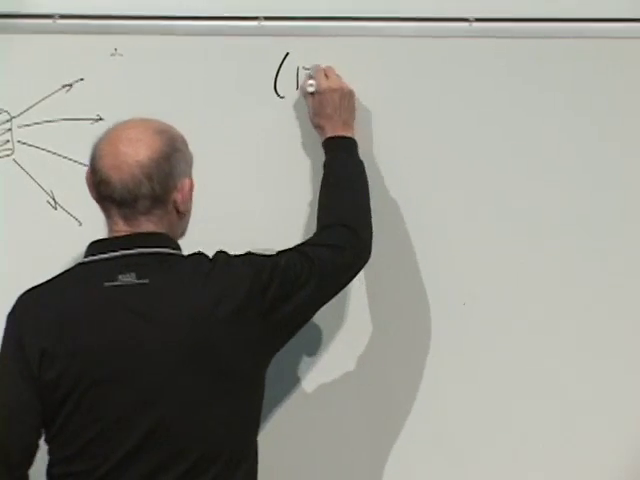
\includegraphics[width=0.66\textwidth]{lecture_06_figure_02.png}
  \caption{La condition de couche de masse dans la convention de métrique utilisée tout au long du cours.}
  \lectureframe{00:05:56}
  \label{fig:l06-mass-shell}
\end{figure}

Considérons deux particules incidentes d’impulsions \(k_1,k_2\) et deux particules émergentes d’impulsions physiques \(q_3,q_4\). La conservation de l’énergie et de l’impulsion s’écrit sous la forme d’une équation unique de quadrivecteurs,
\begin{equation}
  k_1+k_2=q_3+q_4.
  \label{eq:l06-physical-conservation}
\end{equation}
Il est commode d’attribuer une impulsion entrante à chaque ligne externe :
\begin{equation}
  k_3\equiv-q_3,
  \qquad
  k_4\equiv-q_4.
\end{equation}
On a alors
\begin{equation}
  k_1+k_2+k_3+k_4=0,
  \label{eq:l06-all-incoming}
\end{equation}
et chaque ligne vérifie \(k_i^2=-m_i^2\). Les particules émergentes n’ont une énergie négative que dans cette convention de comptabilité ; leurs énergies physiques restent positives.

\begin{figure}[H]
  \centering
  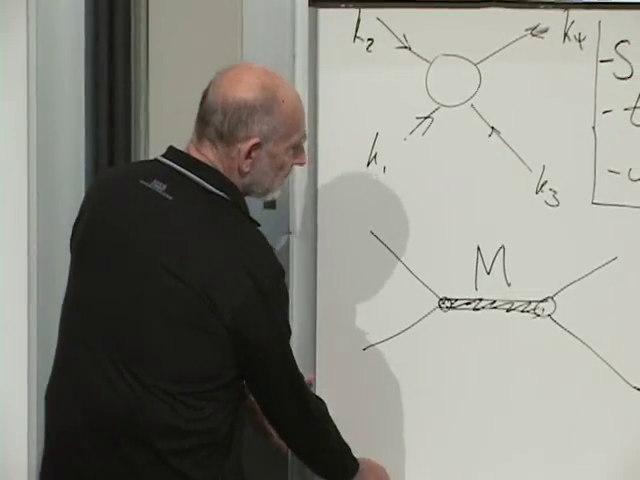
\includegraphics[width=0.68\textwidth]{lecture_06_figure_03.png}
  \caption{On inverse les impulsions physiques des particules émergentes afin de traiter symétriquement comme entrantes les quatre impulsions externes.}
  \lectureframe{00:09:10}
  \label{fig:l06-all-incoming-board}
\end{figure}

Au premier abord, l’amplitude semble être une fonction de seize composantes, \(\mathcal A(k_1,k_2,k_3,k_4)\). La plupart sont redondantes. Passons dans le référentiel du centre de masse, orientons les impulsions incidentes selon un axe choisi et supposons, pour simplifier, que les quatre particules ont la même masse. L’état incident est alors déterminé par un seul nombre : l’énergie du centre de masse. Les impulsions spatiales des particules émergentes doivent être opposées, de même norme, et leur norme doit être égale à celle des impulsions incidentes. Seul leur angle de déflexion \(\theta\) reste à préciser. Le processus dépend donc de deux variables cinématiques indépendantes : \begin{equation}
  E_{\mathrm{cm}},
  \qquad
  \theta.
  \label{eq:l06-two-data}
\end{equation}

\section{Variables de Mandelstam}

Les deux quantités physiques de \eqref{eq:l06-two-data} doivent pouvoir s’exprimer sans choisir de référentiel. Avec la convention où toutes les impulsions sont entrantes, définissons
\begin{equation}
  \begin{aligned}
    -s&=(k_1+k_2)^2,\\
    -t&=(k_1+k_3)^2,\\
    -u&=(k_1+k_4)^2.
  \end{aligned}
  \label{eq:l06-mandelstam}
\end{equation}
Dans le référentiel du centre de masse, les parties spatiales de \(k_1+k_2\) s’annulent ; on a donc
\begin{equation}
  s=E_{\mathrm{cm}}^2.
  \label{eq:l06-s-energy}
\end{equation}

Pour une impulsion physique sortante \(q_3=-k_3\),
\begin{equation}
  k_1+k_3=k_1-q_3
\end{equation}
est l’impulsion transférée de la ligne 1 à la ligne 3. Pour des masses externes égales et une norme \(p\) de l’impulsion spatiale incidente,
\begin{equation}
  -t=2p^2(1-\cos\theta),
  \qquad
  -u=2p^2(1+\cos\theta).
  \label{eq:l06-tu-angle}
\end{equation}
Ainsi, \(t\) et \(u\) portent l’information angulaire mesurée par les détecteurs.

\begin{figure}[H]
  \centering
  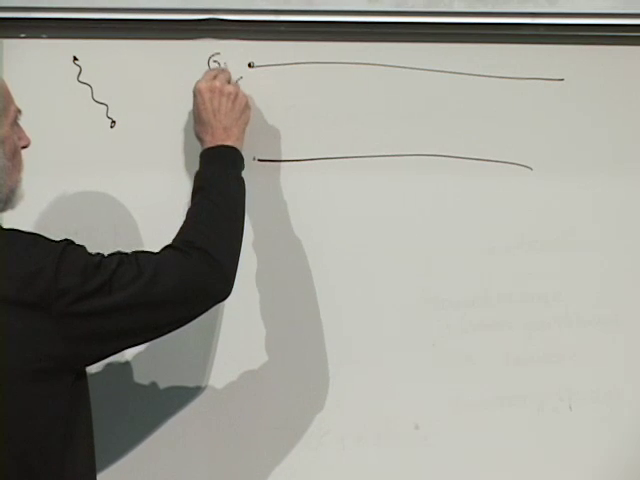
\includegraphics[width=0.74\textwidth]{lecture_06_figure_04.png}
  \caption{Les définitions symétriques de \(s,t,u\) dans la convention où toutes les impulsions sont entrantes.}
  \lectureframe{00:26:20}
  \label{fig:l06-stu-board}
\end{figure}

Trois symboles ne signifient pas qu’il y ait trois données indépendantes. En élevant \eqref{eq:l06-all-incoming} au carré et en utilisant \(k_i^2=-m^2\), on obtient
\begin{equation}
  s+t+u=4m^2
  \label{eq:l06-stu-constraint}
\end{equation}
pour des masses égales. Dès que \(s\) et \(t\) sont connus, \(u\) est fixé.

\begin{classroomqa}
\audiencequestion{Le vide peut-il ralentir une particule en mouvement libre, un peu comme le ferait un frottement ? \lecturetimestamp{00:27:17}}
\lecturerresponse{Pas dans un vide invariant par translation. Il n’y a nulle part où transférer l’impulsion manquante ; la conservation de l’impulsion interdit donc un tel frottement. On peut imaginer un milieu ou un autre vide qui sélectionne un référentiel de repos privilégié, mais ce n’est pas le vide considéré ici.}
\end{classroomqa}

\begin{classroomqa}
\audiencequestion{Pourquoi les deux particules émergentes doivent-elles avoir la même énergie ? \lecturetimestamp{00:27:54}}
\lecturerresponse{Dans le référentiel du centre de masse, leurs impulsions spatiales doivent être opposées et de même norme. Pour le processus à masses égales considéré ici, l’égalité des normes des impulsions entraîne l’égalité des énergies par \(E^2=p^2+m^2\). Si les masses des particules émergentes étaient différentes, cette dernière conclusion devrait être modifiée.}
\end{classroomqa}

\section{Voies directe et croisée}

Dans un diagramme simple de particules ponctuelles, les particules 1 et 2 forment une particule intermédiaire de masse \(M\), qui se désintègre ensuite en 3 et 4. À des facteurs de numérateur et à la prescription de pôles près, la dépendance caractéristique est
\begin{equation}
  \mathcal A_s\sim\frac{g^2}{s-M^2}.
  \label{eq:l06-s-channel}
\end{equation}
C’est le processus de la voie directe, ou voie \(s\). En faisant pivoter la connectivité, on obtient un échange entre les deux lignes externes,
\begin{equation}
  \mathcal A_t\sim\frac{g^2}{t-M^2},
  \label{eq:l06-t-channel}
\end{equation}
qui correspond au processus de la voie croisée, ou voie \(t\). Une troisième connectivité donne
\begin{equation}
  \mathcal A_u\sim\frac{g^2}{u-M^2}.
  \label{eq:l06-u-channel}
\end{equation}

\begin{figure}[H]
  \centering
  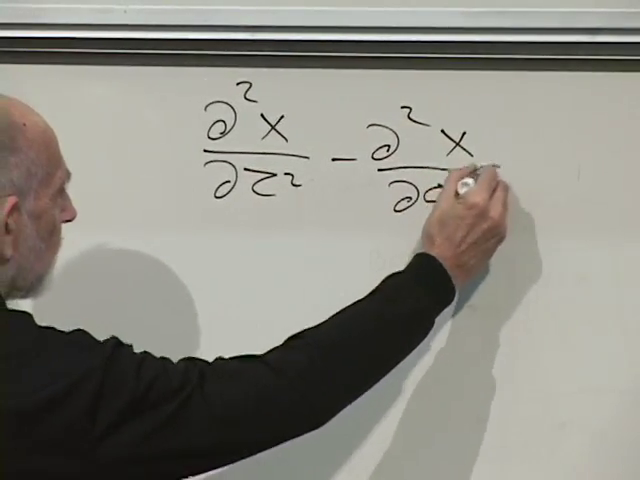
\includegraphics[width=0.72\textwidth]{lecture_06_figure_05.png}
  \caption{Production directe par un état intermédiaire et le pôle correspondant \(g^2/(s-M^2)\) ; la connectivité croisée est représentée sur le même tableau.}
  \lectureframe{00:30:50}
  \label{fig:l06-channel-board}
\end{figure}

La distinction est physique. À ce niveau très rudimentaire, où l’on ne considère que des scalaires, \eqref{eq:l06-s-channel} dépend de l’énergie de collision, mais pas de l’angle. Avant de se désintégrer, l’état composé a perdu la mémoire de la direction incidente ; sa désintégration est donc isotrope. L’amplitude d’échange dépend du transfert d’impulsion et, par conséquent, de l’angle ; une particule échangée légère favorise fortement les faibles déflexions. Le spin ajouterait d’autres dépendances angulaires, mais la structure des pôles est déjà visible.

\begin{classroomqa}
\audiencequestion{La voie \(u\) manquante donne-t-elle un troisième terme ? \lecturetimestamp{00:34:47}}
\lecturerresponse{Oui, dès lors que l’identité des particules et les couplages permettent cette connectivité. On ajoute alors un terme qui présente un pôle en \(u=M^2\). Il ne s’agit pas d’une nouvelle variable cinématique indépendante, puisque \(s+t+u=4m^2\), mais d’un diagramme de canal distinct.}
\end{classroomqa}

\section{Une fonction, deux descriptions de canal}

Un pôle unique décrit mal la diffusion des mésons. Deux mésons peuvent former de nombreuses résonances, avec toute une série de masses et de moments angulaires. Dans les 1960, la première réaction a consisté à ajouter des pôles de la voie \(s\), puis de la voie \(t\), ainsi que les pôles autorisés de la voie \(u\). On a ensuite découvert une fonction bien plus économique. Dans les unités du cours, où la trajectoire de Regge linéaire et son intercept ont été absorbés dans \(s\) et \(t\), elle s’écrit
\begin{equation}
  \mathcal A_{\mathrm V}(s,t)
  \propto
  \frac{\Gamma(-s)\Gamma(-t)}{\Gamma(-s-t)}.
  \label{eq:l06-veneziano}
\end{equation}
La fonction gamma prolonge la factorielle :
\begin{equation}
  \Gamma(n)=(n-1)!
\end{equation}
pour les entiers positifs.

\begin{figure}[H]
  \centering
  \includegraphics[width=0.68\textwidth]{lecture_06_figure_06.png}
  \caption{L’amplitude de Veneziano écrite sous la forme d’un rapport symétrique de fonctions gamma.}
  \lectureframe{00:42:25}
  \label{fig:l06-veneziano-board}
\end{figure}

Les pôles de \(\Gamma(-s)\) reproduisent une série infinie de résonances dans la voie directe. Pourtant, la même expression est symétrique sous \(s\leftrightarrow
t\) ; ses pôles \(\Gamma(-t)\) donnent donc un développement dans la voie croisée. Il ne s’agit pas de deux contributions ajoutées séparément. Une seule fonction analytique admet l’une ou l’autre description. C’est l’ancienne idée de la dualité entre les résonances de la voie directe et les échanges de la voie croisée.

\begin{classroomqa}
\audiencequestion{Comment une amplitude unique peut-elle contenir les deux sommes de canaux sans les additionner ? \lecturetimestamp{00:43:32}}
\lecturerresponse{C’est précisément là que réside la surprise. Le développement de la fonction au voisinage de ses pôles dans la voie \(s\) l’organise en résonances directes ; son développement au voisinage de ses pôles dans la voie \(t\) organise cette même fonction en échanges. Il faut un modèle microscopique pour expliquer pourquoi ces deux lectures coïncident : ce modèle est une corde en interaction.}
\end{classroomqa}

\section{Une bande balayée par une corde ouverte}

Paramétrons une corde ouverte par
\begin{equation}
  0\leq\sigma\leq\pi.
\end{equation}
Le paramètre \(\sigma\) ne désigne pas une position dans l’espace-temps. L’application \(X^\mu(\sigma,\tau)\) indique où se trouve dans l’espace-temps le point ainsi repéré, tandis que \(\tau\) mesure l’évolution. Une particule ponctuelle balaie une ligne d’univers ; la corde en mouvement balaie une feuille d’univers bidimensionnelle. Dans la théorie libre, chaque coordonnée de l’application vérifie
\begin{equation}
  \frac{\partial^2X^\mu}{\partial\tau^2}
  -
  \frac{\partial^2X^\mu}{\partial\sigma^2}
  =0.
  \label{eq:l06-wave-equation}
\end{equation}

\begin{figure}[H]
  \centering
  \includegraphics[width=0.70\textwidth]{lecture_06_figure_07.png}
  \caption{L’équation d’onde qui régit chacune des coordonnées de la corde libre sur la bande de la feuille d’univers.}
  \lectureframe{00:49:10}
  \label{fig:l06-wave-equation-board}
\end{figure}

Pour construire la diffusion, il est utile de ne pas prendre trop tôt la limite continue. Remplaçons chaque corde par \(n\) points matériels reliés par des ressorts. La feuille d’univers devient un ensemble dense de lignes d’univers proches les unes des autres, et ses modes normaux sont de simples oscillateurs harmoniques. Deux chaînes incidentes peuvent se toucher par leurs extrémités. À cet instant, un nouveau ressort les relie ; elles évoluent pendant une durée \(\tau\) comme une chaîne plus longue, puis un ressort se rompt et deux chaînes émergentes se forment à nouveau.

\begin{figure}[H]
  \centering
  \includegraphics[width=0.72\textwidth]{lecture_06_figure_08.png}
  \medskip

  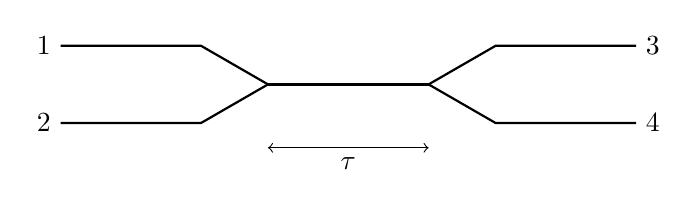
\begin{tikzpicture}[x=0.85cm,y=0.70cm]
    \draw[thick] (0,2.2) -- (2.1,2.2) -- (3.1,1.5);
    \draw[thick] (0,0.8) -- (2.1,0.8) -- (3.1,1.5);
    \draw[thick] (3.1,1.5) -- (5.5,1.5);
    \draw[thick] (5.5,1.5) -- (6.5,2.2) -- (8.6,2.2);
    \draw[thick] (5.5,1.5) -- (6.5,0.8) -- (8.6,0.8);
    \draw[<->] (3.1,0.35) -- node[below] {\(\tau\)} (5.5,0.35);
    \node[left] at (0,2.2) {1};
    \node[left] at (0,0.8) {2};
    \node[right] at (8.6,2.2) {3};
    \node[right] at (8.6,0.8) {4};
  \end{tikzpicture}
  \caption{Deux cordes ouvertes discrétisées se touchent, forment une seule corde intermédiaire pendant une durée \(\tau\), puis se séparent. Le cadre source conserve la construction en ressorts et en lignes d’univers ; le schéma met en évidence leurs connexions.}
  \lectureframe{00:51:25}
  \label{fig:l06-string-joining}
\end{figure}

Les deux cordes ne sont dessinées côte à côte que dans l’espace des paramètres. Leurs positions dans l’espace-temps n’ont pas besoin d’être voisines tant que les coordonnées de leurs extrémités ne coïncident pas effectivement. La liberté de reparamétrisation permet de placer les événements de jonction et de séparation à des positions commodes dans le diagramme ; cette liberté géométrique deviendra la symétrie conforme dans le cours suivant.

\section{Le calcul des oscillateurs, étape par étape}

Désignons les coordonnées de la première chaîne par \(x_1,\ldots,x_n\) et celles de la seconde par \(x_{n+1},\ldots,x_{2n}\). Leurs coordonnées de centre de masse sont
\begin{equation}
  X_{\mathrm{cm}}^{(1)}
  =\frac1n\sum_{a=1}^{n}x_a,
  \qquad
  X_{\mathrm{cm}}^{(2)}
  =\frac1n\sum_{a=n+1}^{2n}x_a.
  \label{eq:l06-chain-centers}
\end{equation}
Une chaîne d’impulsion déterminée \(k_1\) possède une onde plane de centre de masse multipliée par l’état fondamental de ses oscillateurs internes :
\begin{align}
  \Psi_1
  &=
  e^{ik_1\cdot X_{\mathrm{cm}}^{(1)}}
  \psi_0(x_1,\ldots,x_n),
  \\
  \Psi_2
  &=
  e^{ik_2\cdot X_{\mathrm{cm}}^{(2)}}
  \psi_0(x_{n+1},\ldots,x_{2n}).
  \label{eq:l06-two-wavefunctions}
\end{align}
Les facteurs \(\psi_0\) dépendent des coordonnées relatives et non de la translation commune de toute la chaîne. Comme les cordes incidentes constituent initialement des systèmes quantiques distincts,
\begin{equation}
  \Psi_{\mathrm{in}}=\Psi_1\Psi_2.
  \label{eq:l06-product-state}
\end{equation}

\begin{figure}[H]
  \centering
  \includegraphics[width=0.76\textwidth]{lecture_06_figure_09.png}
  \caption{Les deux ondes planes d’impulsion et leurs facteurs d’état fondamental des oscillateurs internes, représentés dans des couleurs distinctes.}
  \lectureframe{00:58:05}
  \label{fig:l06-wavefunctions-board}
\end{figure}

La jonction sélectionne la partie de cette fonction d’onde pour laquelle les coordonnées des deux extrémités coïncident :
\begin{equation}
  x_n=x_{n+1}.
  \label{eq:l06-endpoint-contact}
\end{equation}
À cet instant, les autres coordonnées restent inchangées. L’état sélectionné évolue alors sous l’action de l’hamiltonien \(H_{\mathrm{joined}}\) de la chaîne unique plus longue :
\begin{equation}
  \Psi(\tau)
  =
  e^{-iH_{\mathrm{joined}}\tau}\Psi(0).
  \label{eq:l06-time-evolution}
\end{equation}
Enfin, on calcule son recouvrement avec un produit d’états de cordes émergentes, d’impulsions \(q_3,q_4\).

\begin{figure}[H]
  \centering
  \includegraphics[width=0.76\textwidth]{lecture_06_figure_10.png}
  \caption{La fonction d’onde des deux chaînes juste avant d’imposer la coïncidence de leurs extrémités.}
  \lectureframe{00:58:55}
  \label{fig:l06-endpoint-board}
\end{figure}

Le calcul est long, mais il n’a rien de mystérieux. Chaque coordonnée interne peut être décomposée en modes oscillatoires ; le recouvrement à la jonction, l’évolution temporelle et la projection finale se ramènent donc à de l’algèbre gaussienne des oscillateurs. La durée \(\tau\) pendant laquelle la corde reste jointe est la seule quantité qui ne soit pas fixée.

\begin{classroomqa}
\audiencequestion{Les fonctions d’onde noire et rouge s’additionnent-elles ou se multiplient-elles ? \lecturetimestamp{01:02:26}}
\lecturerresponse{Elles se multiplient. Dans la représentation en coordonnées, l’état produit tensoriel de deux systèmes indépendants est représenté par le produit de leurs fonctions d’onde. Une somme décrirait une superposition de possibilités, et non la présence simultanée des deux cordes incidentes.}
\end{classroomqa}

\begin{classroomqa}
\audiencequestion{Pourquoi intégrer sur le temps intermédiaire \(\tau\) ? \lecturetimestamp{01:04:04}}
\lecturerresponse{On n’attribue pas de durée fixe à la corde jointe. La règle de Feynman consiste à sommer les amplitudes sur toutes les histoires possibles. Dans cette description, le paramètre continu restant pour caractériser l’histoire est la durée entre la jonction et la séparation ; la somme devient donc une intégrale sur \(0\leq\tau<\infty\).}
\end{classroomqa}

\section{Du temps de propagation à la fonction bêta}

Après le calcul des recouvrements des oscillateurs, le résultat peut s’écrire sous la forme
\begin{equation}
  \mathcal A(s,t)
  \propto
  \int_0^\infty d\tau\,
  e^{\tau(s+1)}
  \bigl(1-e^{-\tau}\bigr)^{-t-1}
  e^{-\tau}.
  \label{eq:l06-tau-integral}
\end{equation}
On laisse apparaître le facteur final \(e^{-\tau}\), car il fournit le jacobien nécessaire à l’étape suivante. De façon équivalente, les exponentielles de début et de fin se regroupent en \(e^{s\tau}\).

\begin{figure}[H]
  \centering
  \includegraphics[width=0.76\textwidth]{lecture_06_figure_11.png}
  \caption{L’intégrande en fonction du temps de propagation après le calcul des oscillateurs ; le facteur distinct \(e^{-\tau}\) fournit le jacobien du changement de variable.}
  \lectureframe{01:06:45}
  \label{fig:l06-tau-integral-board}
\end{figure}

Posons maintenant
\begin{equation}
  z=e^{-\tau},
  \qquad
  dz=-e^{-\tau}\,d\tau.
  \label{eq:l06-z-substitution}
\end{equation}
Quand \(\tau\) varie de \(0\) à \(\infty\), \(z\) varie de \(1\) à \(0\). Le signe moins inverse les bornes, d’où
\begin{equation}
  \mathcal A(s,t)
  \propto
  \int_0^1
  z^{-s-1}(1-z)^{-t-1}\,dz.
  \label{eq:l06-beta-integral}
\end{equation}

\begin{figure}[H]
  \centering
  \includegraphics[width=0.74\textwidth]{lecture_06_figure_12.png}
  \caption{Le changement de variable \(z=e^{-\tau}\) fait apparaître l’intégrale bêta d’Euler.}
  \lectureframe{01:08:49}
  \label{fig:l06-beta-integral-board}
\end{figure}

Cette intégrale est définie directement lorsque ses bornes convergent, et ailleurs par prolongement analytique. C’est la fonction bêta d’Euler :
\begin{equation}
  B(-s,-t)
  =
  \frac{\Gamma(-s)\Gamma(-t)}{\Gamma(-s-t)}.
  \label{eq:l06-beta-gamma}
\end{equation}

\begin{figure}[H]
  \centering
  \includegraphics[width=0.72\textwidth]{lecture_06_figure_13.png}
  \caption{Le tableau identifie l’intégrale transformée à \(B(-s,-t)\) et commence à rétablir son expression en fonctions gamma.}
  \lectureframe{01:12:24}
  \label{fig:l06-beta-gamma-board}
\end{figure}

La symétrie entre les voies est maintenant élémentaire. Sous \(z\mapsto1-z\),
\begin{equation}
  \int_0^1 z^{-s-1}(1-z)^{-t-1}\,dz
  =
  \int_0^1 z^{-t-1}(1-z)^{-s-1}\,dz.
\end{equation}
On a donc \(\mathcal A(s,t)=\mathcal A(t,s)\). Un processus construit à partir de deux cordes qui se rejoignent puis se séparent contient automatiquement aussi la description croisée.
\editorialnote{Dans les arguments de la fonction bêta, le cours omet la pente de Regge et l’intercept. Dans la notation standard, on remplace \(s,t\) par les trajectoires linéaires correspondantes \(\alpha(s),\alpha(t)\). La dualité et l’argument fondé sur le changement de variable restent inchangés.}

\begin{classroomqa}
\audiencequestion{Le rapport de fonctions gamma ressemble aux expressions factorielles rencontrées en combinatoire. Existe-t-il une interprétation directe en termes de dénombrement physique ? \lecturetimestamp{01:13:22}}
\lecturerresponse{Pour des arguments entiers, la fonction bêta est liée à un rapport tel que \(n!\,m!/(n+m)!\), mais rien n’affirme ici l’existence d’un mécanisme combinatoire. La même fonction spéciale apparaît dans l’intégrale sur la feuille d’univers ; cette ressemblance n’est pas à l’origine de l’amplitude.}
\end{classroomqa}

La raison, encore cachée, pour laquelle on peut lire une même feuille d’univers dans les deux voies est la symétrie conforme. Elle permet d’étirer la feuille comme de la pâte sans modifier l’amplitude, transformant une longue région de propagation dans la voie directe en une représentation par échange dans la voie croisée. Cette explication géométrique est reportée au cours suivant.

\section{Ce que l’étude de la diffusion a établi}
\enlargethispage{3\baselineskip}
\begingroup
\setlength{\medskipamount}{3pt plus 1pt minus 1pt}

La représentation discrète de la jonction a suscité une dernière série de questions.

\begin{classroomqa}
\audiencequestion{Si deux chaînes de \(n\) constituants se rejoignent par leurs extrémités, le résultat contient-il \(2n-1\) constituants, et cela pourrait-il modifier la parité fermionique ? \lecturetimestamp{01:16:16}}
\lecturerresponse{Dans la représentation hadronique des extrémités, on peut considérer la paire d’extrémités qui se touchent comme une paire particule-antiparticule qui s’annihile ; le nombre diminue donc de deux, et non d’une unité. Dans la limite continue, la différence finie entre \(2n\) et \(2n-2\) est sans importance, mais la conservation de la parité fermionique, elle, ne l’est pas. Les constituants du réseau ne sont qu’un régulateur de la corde continue, et non des grains fondamentaux au sens littéral.}
\end{classroomqa}

\begin{classroomqa}
\audiencequestion{La suite du cours abordera-t-elle les mathématiques complètes des supercordes ? \lecturetimestamp{01:18:05}}
\lecturerresponse{Seules certaines conséquences seront utilisées. La suite immédiate passe par la symétrie de la feuille d’univers et la compactification, puis par un autre point de départ, élaboré au milieu des années 1990s : la théorie M. Son objectif est de retrouver la même physique à partir d’un point de vue qui rend transparentes plusieurs caractéristiques autrement complexes.}
\end{classroomqa}

\begin{classroomqa}
\audiencequestion{Cette règle de jonction n’était-elle qu’un indice tiré des collisions de mésons ? \lecturetimestamp{01:20:02}}
\lecturerresponse{La diffusion des mésons a fourni l’indice historique, mais la règle s’applique de façon générale aux cordes ouvertes. La même topologie décrit les collisions de photons de corde ouverte et d’autres états de corde ouverte. Deux cordes fermées se rejoignent et se séparent selon une construction analogue, avec une corde fermée dans la région intermédiaire.}
\end{classroomqa}

\begin{classroomqa}
\audiencequestion{Le calcul ne s’applique-t-il qu’aux états de corde fermioniques ? \lecturetimestamp{01:20:56}}
\lecturerresponse{Non. Le calcul original de Veneziano concerne la corde ouverte bosonique. Les supercordes exigent des degrés de liberté fermioniques supplémentaires et modifient certains détails de l’intégrande, mais la logique de jonction, de propagation, de projection et de dualité sur la feuille d’univers reste très analogue.}
\end{classroomqa}

La présence d’un état de spin un ou deux dans le spectre des oscillateurs était suggestive, mais ne constituait pas une preuve décisive. Les amplitudes de diffusion correspondantes ont fourni un test plus probant. Les amplitudes des photons satisfont les identités associées à la conservation de la charge et à l’invariance de jauge ; celles des gravitons satisfont les contraintes correspondantes d’un champ sans masse de spin deux. Les états de la corde ont satisfait ces tests dans leurs interactions entre eux, ainsi qu’avec des états massifs et sans masse. C’est pourquoi les appellations de photon et de graviton sont devenues des identifications physiques plutôt que de simples hypothèses fondées sur le dénombrement des polarisations.
\editorialnote{Dans le langage moderne, ces tests s’expriment par le découplage des polarisations non physiques, les identités de Ward de jauge et le couplage universel à basse énergie de l’état sans masse de spin deux.}

\begin{classroomqa}
\audiencequestion{D’où vient la charge électrique elle-même dans la description par les cordes ? \lecturetimestamp{01:24:03}}
\lecturerresponse{Le cours s’achève sans répondre à cette question. La réponse exige de connaître la structure interne et la structure des extrémités de la théorie des cordes, qui n’ont pas encore été introduites ; elle relève donc de la suite du cours plutôt que de cette dérivation de la diffusion.}
\end{classroomqa}
\endgroup
